% vim:tw=80 ts=2 et sw=2 indentexpr= :
\documentclass[a4paper,12pt]{scrartcl}
\usepackage[utf8]{inputenc}
\usepackage[T1]{fontenc}
\usepackage[ngerman]{babel}
\usepackage{libertine} % kann man notfalls auch ignorieren, wenns nicht da ist
\usepackage{textcomp} % notfalls für €
\usepackage{stratum0doc}
\usepackage[colorlinks=false]{hyperref}
\usepackage{graphicx}
\usepackage{savefnmark}

\title{3.~Mitgliederversammlung des Stratum~0~e.~V.}
\date{16.~März~2013}

\begin{document}
\maketitle
{\footnotesize\tableofcontents}

%%%%%%%%%%%
%% TOP 0 %%
%%%%%%%%%%%
\section{Organisatorischer Overhead}
\begin{description}
  \item[Zeit:] 16. März 2013, 20:00
  \item[Ort:] TanzSportZentrum Braunschweig, Hamburger Straße 273a
  \item[Anwesend:] 20 von 65 Mitgliedern (30{,}7\%), Versammlung ist somit
  beschlussfähig. 2 Gäste durch die Versammlung ohne Einwände zugelassen.
  \item[Wahl des Versammlungsleiters:] Vincent Breitmoser einstimmig durch
    Handzeichen; nimmt die Wahl an
  \item[Protokoll:] Roland Hieber einstimmig durch Handzeichen, nimmt die Wahl
    an.
  \item[Veranstaltung eröffnet] durch den Versammlungsleiter um 20:05
	\item[Tagesordnung:] ohne Gegenstimmen angenommen.
\end{description}

\paragraph{Anträge zur Geschäftsordnung}
Die Veranstaltung beschließt auf Antrag einstimmig, bei einer klaren Mehrheit
für einen Antrag zur Vereinfachung keine genauen Abstimmungsergebnisse
festzustellen, sondern nur die Anzahl der Gegenstimmen und Enthaltungen.

\paragraph{Kurzer Bericht des Vorstandes}
Da seit der letzten Mitgliederversammlung nur wenig Zeit vergangen ist, fällt
der Bericht des Vorstandes durch den Vorstandsvorsitzenden verhältnismäßig kurz
aus. Der neu gewählte Vorstand war hauptsächlich mit Notarbesuchen und weiteren
Formalitäten beschäftigt.


%%%%%%%%%%%
%% TOP 1 %%
%%%%%%%%%%%
\section{Kapuzenpullover\label{sec:pullover}}
Die T-Shirts mit dem Vereinslogo, die im März 2012 bei Hönkeldruck bestellt
wurden, wurden gut angenommen, und es war im Gespräch, bei der nächsten
Bestellung auch Pullover und Zipper-Hoodies zu bestellen. Nachdem auf der
Vorstandssitzung am 3. Juni 2012\footnote{Protokoll:
\url{https://stratum0.org/wiki/Datei:Vorstandssitzung_2012-06-03.pdf}}
beschlossen wurde, bei T-Shirts auf weitere Vorbestellungen zu warten und auch
nach vorhandenem Bedarf Pullover zu bestellen, wurde im November 2012 dann eine
neue Bestellung aufgegeben, wobei Julien Deseke mit Hönkeldruck in Kontakt
stand.  Hönkeldruck lieferte nun am 13. März 2013 die Bestellung aus, es waren
aber außer den bestellten 37 T-Shirts nun auch gleich 15 Unisex-Pullover zu je
21€ und 15 Girly-Pullover zu je 20€ dabei, wobei zu dem Zeitpunkt höchstens 3
Mitglieder Interesse an (Unisex-)Pullovern gezeigt hatten. Es stellte sich
heraus, dass zwischen dem Vorstand und Julien sowie zwischen Julien und
Hönkeldruck Kommunikationsfehler auftraten, die zu der hohen Menge an Pullovern
führten. 

\consensus{Julien Deseke tritt als Beisitzer im Vorstand zurück}
Nun steht der Verein vor dem Problem, ein Kapital von 573€ in 28 bestellten,
aber nicht benötigten Pullovern angelegt zu haben. Eine Rückgabe an Hönkeldruck
ist sehr wahrscheinlich ausgeschlossen, da sie nunmal (wenn auch ohne
Legitimierung durch den Vorstand) bestellt wurden, und da es sich um individuell
angefertige Kleidungsstücke handelt. Angesichts der Tatsache, dass die
Mitgliederversammlung in einem späteren Tagesordnungspunkt eine Entscheidung
über 6000€ für neue Räumlichkeiten fällen soll, und um den restlichen Vorstand
nicht in Misskredit zu bringen, nimmt Julien die Verantwortung für die
Misskommunikation auf sich und stellt sein Amt als Beisitzer mit sofortiger
Wirkung zur Verfügung. Damit verbleiben in dieser Wahlperiode nach §8, Abs.~1
der Satzung vorerst nur zwei weitere Beisitzer im Vorstand.

Da die Pullover mit Girly-Schnitt voraussichtlich weniger nachgefragt werden,
hat der Vorstand beschlossen, diese Pullover zu subventionieren, und den
Unterschied auf die Pullover mit Unisex-Schnitt aufzuschlagen (Vincent bemerkt
an der Stelle, dass der Girly-Schnitt auch an männlichen Entitäten sehr bequem
sitzt). Zusätzlich haben zum Glück auch schon 7 Personen aus dem shackspace in
Stuttgart Interesse an Pullovern angemeldet. Die bestellten T-Shirts werden
wiederum schon häufig nachgefragt, jedoch sind sie gegenüber den Pullovern auch
um einiges günstiger.


%%%%%%%%%%%
%% TOP 2 %%
%%%%%%%%%%%
\section{Miete einer neuen Räumlichkeit}

Der Verein steht im Moment vor dem Problem, viel zu viel Geld und viel zu wenig
Platz zur Verfügung zu haben. In den aktuellen Räumlichkeiten ist schon bei
Vorträgen wenig Platz und Entitäten treten sich auf die Zehen. Insbesondere
fehlt Platz, um größere Geräte (Lasercutter, Stickmaschine, CNC-Fräse, Werkbank,
etc.) anzuschaffen und damit die in der Satzung formulierten Vereinsziele zu
erfüllen. Diesem Umstand könnte aber demnächst abgeholfen werden, da ein Makler
von nowo dem Verein vor etwa einem Monat ein Angebot für weitere Räumlichkeiten
im selben Gebäude gemacht hat, die zur Zeit leer stehen und 140m$^2$ umfassen.
Als Kaltmiete werden vom Makler 350€ angesetzt, was in etwa der aktuell vom
Verein gezahlten Miete entspricht. Der Haken dabei ist allerdings, dass es sich
im Wesentlichen um zwei blanke Räume ohne vorhandene Infrastruktur (insbesondere
ohne Bad bzw.  Wasseranschluss) handelt, die auf Kosten des Vereins renoviert
werden müssten, um den Komfort der aktuellen Räumlichkeiten nicht zu verlieren.
Diese sollen dann im Laufe des Umzugs gekündigt werden.

Es gab darauf hin mehrere Besichtigungstermine, damit sich die Mitglieder ein
Bild von der Räumlichkeit machen konnten, Fotos wurden im Wiki
bereitgestellt\footnote{siehe
\url{https://stratum0.org/wiki/Arbeitsgruppe:Space_v2.0}}. Außerdem gab es
drei Planungstreffen, auf denen der Umbau der Räumlichkeit durch interessierte
Mitglieder geplant wurde. Diese Arbeitsgruppe hat nun mehrere Optionen sowie
Aufwandsschätzungen ausgearbeitet, die von reneger und chrissi\^{} in einer
Präsentation (siehe \ref{sec:praesentation}) und einer Kalkulationstabelle
(siehe \ref{sec:kostenplanung}) präsentiert werden.

Zusätzlich wurde von der Arbeitsgruppe die augenscheinlich vorhandene
Feuchtigkeit der Außenwand als KO-Kriterium definiert. Falls dieses Problem
nicht gelöst werden kann, werden die neuen Räumlichkeiten nicht angemietet. Des
Weiteren gilt, was auch immer hier beschlossen wird, nur umgesetzt wird, sofern
der Vermieter zustimmt.

Nach der Präsentation der Planung werden noch Fragen beantwortet und durch die
Arbeitsgruppe beantwortet.

\question{Wie ist Mitgliederentwicklung, sind die neuen Räumlichkeiten
vielleicht auch bald zu klein?}
\answer{Bisher 1{,}5 bis 2 neue Mitglieder pro Monat, die
Mitgliederentwicklung ist etwa logarithmisch. Außerdem ist das aktuelle Angebot
ziemlich günstig für uns und kommt nicht in nächster Zeit sehr wahrscheinlich
nicht wieder.}

\question{Was passiert im Worst Case, wenn alle Sponsoren wegbrechen und 10
Mitglieder austreten?}
\answer{Siehe Präsentation, Folie 10. Die Rechnung dort ist sehr konservativ.}

\question{Was ist mit der Belüftung im Frickelraum? Das Fenster dort lässt sich
nicht öffnen.}
\answer{Deswegen gibt es die Fenster in der Zwischenwand, als Alternative bietet
sich ein Lüfter im Fenster an.}

\question{Könnte man ein zusätzliches Fenster in die Wand im Frickelraum bauen?}
\answer{Mehrkosten dafür wären etwa 150€, es braucht die Zustimmung des
Vermieters.}

\question{Könnte man zwei Monate warten, um noch mehr Mitgliedsbeiträge
einzunehmen?}
\answer{Das wird eh der Fall sein durch die Zeit während der Renovierung.}

\question{Was für eine Duschwanne wird eingebaut?}
\answer{Die Duschwanne ist voraussichtlich eine barrierefreie Duschwanne, die in
den Boden integriert ist.}

\question{Könnte man die Tür zum Frickelraum in die Zwischenwand zum Chillraum
bauen statt zur Werkstatt hin?}
\answer{Das wurde in Erwägung gezogen, man müsste aber dann z.~B. Vorträge im
Chillraum stören, um in den Frickelraum zu kommen. In der Wand zur Werkstatt ist
eine zugemauerte Tür vorhanden, die wieder geöffnet wird. Wenn später Geld übrig
bleibt, kann man auch beide Türen einbauen.}

\question{Könnte man die schräge Wand Richtung Westen auf die andere Seite der
Chillraum-Tür verlegen?}
\answer{Nein, die Tür ist zu breit, dann wird die Wand zu schräg.}

\question{Die Arbeitsstunden sind zu gering angesetzt.}
\answer{Ist uns bewusst, es wurden Facharbeiterstunden zugrunde gelegt. Aber wir
zählen eh nicht nach und die Planung hat nicht den Charakter eines
professionellen Kostenvoranschlags.}

\question{Sollte es eine Selbstverpflichtung für Arbeitsstunden geben?}
\answer{Nein.}

\question{Sind genügend Kompetenzen für die Arbeiten vorhanden?}
\answer{Ja, reneger baut grad ein Haus, der kennt sich aus. Andere Mitglieder
können was dabei lernen.}

\question{Wo ist die Hebeanlage in der Kostenplanung berücksichtigt?}
\answer{Die Planung war noch zu kurzfristig, darum ist die Hebeanlage noch nicht
berücksichtigt. Das aktuelle Abwasserrohr hat nur 40~mm Durchbesser, es werden
100~mm für eine funktionierende Toilette benötigt, als Alternative kann man auch
ein größeres Rohr einbauen.}

\question{Die Küche ist sehr schlauchförmig, wäre es nicht besser, stattdessen
den Flur zu vergrößern?}
\answer{Das haben wir auch gedacht, aber das wäre verschwendeter Platz. In der
Küche kann man sich aufhalten und z.~B. eine Bar bei Veranstaltungen machen. Der
Flur ist größer, als es auf dem Grundriss scheint.}

\newpage
\question{Ist der Sicherungskasten im Flur?}
\answer{Ja, neben der Eingangstür Richtung Bad. Der Plan ist da nicht ganz
genau. Es sollte außerdem Flexibilität für die Ausführung des Plan gegeben
sein.}

\question{Wo ist die Zeit für die Möblierung einberechnet?}
\answer{Die Zeit ist als Pauschale enthalten. Sofas runtertragen geht schnell.} 

\question{Gibt es einen Projektplan mit Abhängigkeiten?}
\answer{Höchstens auf großer Detailebene, hängt auch vom Umbau des Abwassers ab.
Die Arbeitsgruppe hat das als nächsten Schritt nach der Mitgliederversammlung
geplant.}

\question{Ab wann werden die Räumlichkeiten angemietet?}
\answer{Das kommt auf den Vermieter und den Beschluss an. 1. April oder 1. Mai
oder später ist denkbar.}

\question{Was ist der Plan, wenn das Geld wirklich alle ist?}
\answer{Dann muss man sich Finanzierungsmöglichkeiten überlegen, oder es läuft
halt langsamer. Wir erwarten keinen stagnierenden Finanzfluss.}

\question{Kann man die Lüftung ins Frickelraumfenster nachträglich einbauen?}
\answer{Ja, dann kommt ein neues Fenster rein. Der Vermieter muss zustimmen.}

Nach einer Pause von 20 Minuten wird zuerst über die Anmietung der neuen
Räumlichkeit, die Umsetzung der Muss-Kriterien und die Kündigung der alten
Räumlichkeit abgestimmt, falls keine KO-Kriterien auftauchen. Ein kurzes,
sehr eindeutiges Meinungsbild über den Abstimmungsmodus ergibt, dass eine
einfache Mehrheit zur Annahme des Beschlusses ausreicht. 

\consensus{Falls keine KO-Kriterien auftreten: Anmietung neuer Räumlichkeiten, 
Umsetzung der Muss-Kriterien, Kündigung alte Räumlichkeiten}
Es nehmen 19 Mitglieder an der Abstimmung teil, bis auf eine Enthaltung stimmen
alle Mitglieder für die Anmietung, die Umsetzung der Muss-Kriterien, und die
Kündigung der alten Räumlichkeiten.

Anschließend wird über die einzelnen Optionen abgestimmt. Ein weiteres
Meinungsbild ergibt, dass auch hier eine einfache Mehrheit ausreicht, um einen
Beschluss zu fassen.

\begin{itemize}
  \item \consensus{Dusche und Boiler einbauen}    
    Für einen Durchlauferhitzer, falls keine Dusche eingebaut wird, stimmen
    alle anwesenden Mitglieder. Für eine Dusche stimmen alle anwesenden
    Mitglieder bis auf 4 Enthaltungen. Es soll also eine Dusche und ein Boiler
    eingebaut werden.
  \item \consensus{Farbe an den Wänden}
    Für das Streichen der Wände mit Wandfarbe gibt es eine Enthaltung, alle
    anderen Mitglieder sind dafür. Die Wände sollen also gestrichen werden.
  \item \consensus{Brüstungskanal einbauen, außer in der Küche}
    Für den Einbau eines Brüstungskanals im Chillraum, Frickelraum und in der
    Werkstatt stimmen alle anwesenden Mitglieder. Es soll also ein
    Brüstungskanal in diesen Räumen eingebaut werden.
  \item \vote{Netzwerkdosen schon jetzt einbauen}{12}{2}{5}
    \enlargethispage{\baselineskip}
    Zur Ausstattung des Brüstungskanals mit Netzwerkdosen wird angemerkt, dass
    hierfür vermutlich einen Sponsor gewinnen könnte. Die Option kann aber
    auch nach dem Umzug verwirklicht werden. Es sprechen sich 12 Mitglieder
    dafür aus, jetzt schon Netzwerkdosen einzubauen, 2 Mitglieder sind dagegen,
    es gibt 5 Enthaltungen. Die Netzwerkdosen sollen also schon mit dem
    Brüstungskanal eingebaut werden.
\end{itemize}

Für den Mietvertrag gibt es mehrere Optionen. Zum einen könnten wir mit einer
Mindestvertragslaufzeit von 3 Jahren bessere Konditionen erreichen als ohne
Mindestlaufzeit, andererseits können wir nicht abschätzen, was in 3 Jahren sein
wird. Generell wird der Vorstand versuchen, so günstig wie möglich zu
verhandeln, und z.~B. auch ein Sonderkündigungsrecht bei Vereinsauflösung zu
erreichen. Im Endeffekt wird also damit über eine Gesamtmiete von 36$\times$350€
= 12\,600€ abgestimmt.

Es wird zuerst darüber abgestimmt, ob ein Mietvertrag mit 3 Jahren
Mindestvertragslaufzeit unterschrieben werden soll. Eine überwältigende Mehrheit
der Mitglieder spricht sich dafür aus. Da einige Mitglieder über die 
Formulierung des Beschlusses verwirrt sind, wird die Abstimmung wiederholt.

Zuerst wird nun darüber abgestimmt, ob der Vorstand einen Mitvertrag
unterschreiben soll, der als hartes Kriterium eine Verpflichtung von 3 Jahren
Mindestmietdauer enthält, aber kein Sonderkündigungsrecht enthält. Falls dieser
Beschluss nicht angenommen wird, soll im Anschluss darüber abgestimmt werden, ob
ein solcher Vertrag mit Mindestmietdauer von 3 Jahren ein Sonderkündigungsrecht
für den Fall der Vereinsauflösung enthalten soll.

\consensus{Mietvertrag mit Mindestemietdauer von 3 Jahren, ohne
Sonderkündigungsrecht}
Es spricht sich die Mehrheit der anwesenden Mitglieder für die erste Option aus,
wobei sich 5 Mitglieder enthalten. Damit entfällt die zweite Abstimmung, und der
Vorstand wird beauftragt, den Mietvertrag mit einer Mindestdauer von 3 Jahren,
aber ohne Sonderkündigungsrecht im Falle einer Vereinsauflösung zu verhandeln.

Ein Antrag, auch über eine Mindestkündigungsfrist abzustimmen, wird von der
Mehrheit der Mitglieder abgelehnt, da dies zu sehr ins Detail geht. Der Vorstand
wird, wie schon erwähnt, versuchen, möglichst die besten Konditionen zu
verhandeln.

Insgesamt wurde also nun entschieden, dass etwa 6000€ aus Vereinsmitteln in die
Renovierung der neuen Räumlichkeit fließen werden. Als nächste Schritte wird der
Mietvertrag ausgehandelt und die Zeitplanung verfeinert. Mögliche Sponsoren und
im Voraus zahlende Mitglieder sollen sich beim Schatzmeister melden.

Eine letzte Frage wird in Bezug auf das neu gegründete FabLab Braunschweig
gestellt. Möglicherweise könnte dieser Verein eine Konkurrenz für uns
darstellen. Es wurde auch schon Kontakt mit ihnen geknüpft, aber wir stellen
aber fest, dass wir das FabLab vorerst keine Relevanz hat, solange sie uns keine
Schlägertrupps vorbeischicken.


%%%%%%%%%%%
%% TOP 3 %%
%%%%%%%%%%%
\section{Sonstiges}
Die Keysigning-Party wird aufgrund der fortgeschrittenen Zeit auf einen späteren
Zeitpunkt vertagt.

\begin{description}
  \item[Versammlung geschlossen] um 22:43
\end{description}


%%%%%%%%%%%%%
%% Anhänge %%
%%%%%%%%%%%%%
\appendix

%%%%%%%%%%%%%%%%%%%%%%%%%%%
%% Vorstellung Space 2.0 %%
%%%%%%%%%%%%%%%%%%%%%%%%%%%
\newcommand{\includepage}[1]{%
  \begin{center}
    \fbox{
      
\includegraphics[%
        height=0.38\textheight,%
        page=#1,%
        bb=29pt 28pt 764pt 591pt,%
        clip=true%
        ]{images/vorstellung-space2-0.pdf}%
    }%
  \end{center}%
}
%\newcommand{\anmerkung}[1]{\footnotesize{#1}}
\newcommand{\anmerkung}[1]{#1}

\cleardoublepage
\section{Präsentation zur Vorstellung des Space 2.0}\label{sec:praesentation}
%\enlargethispage{4\baselineskip}
Mündliche Erklärungen sind nachfolgend zu den einzelnen Folien aufgeführt.

\includepage{1}
\includepage{2}

\includepage{3}
\includepage{4}
\anmerkung{Werkstatt für dreckige Sachen, Lackieren etc. ist relativ wichtig.
Größerer Vortragsraum bietet mehr Platz für Vorträge. Schräge Wand durch Türen
und Fenster bedingt, damit wenigstens etwas Licht in die Räume kommt. Wände sind
Trockenbauwände, damit man auch Schrauben reindrehen kann. Vorhandene Fenster
sind etwa auf Bodenniveau. Küche relativ groß geplant als zusätzliche
Chillout-Zone/Sitzecke.}

\includepage{5}
\anmerkung{Arbeitsaufwand geschätzt ca. 400 Personenstunden, dafür die
Möglichkeit, Infrastruktur nach eigenen Vorstellungen zu schaffen.

Fenster zwischen Chill- und Frickelraum für mehr Licht im Frickelraum.

Brüstungskanal mit Anschlüssen für Strom, Netzwerk, etc.

Wasser/Abwasser: nur je ein zu dünnes Rohr vorhanden, muss verlegt werden;
Boiler oder Durchlauferhitzer für Warmwasser. Planung ist mit Klempner und
Hausmeister gemacht worden, noch ziemlich kurzfristig, möglicherweise Hebeanlage
nötig.

Bodenbelag Chill- und Frickelraum: Nadelfilz, Bad und Küche: Fliesen.

Bad: Waschbecken, Dusche, Abzug gegen Gerüche.

Küche: Dunstabzugshaube inkl. Rohr, gerade wegen Aufenthaltsmöglichkeit in der
Küche wichtig.

Wände: aktuell nur gemauerte Wand, alte Farbe, Putz bröckelt (Feuchtigkeit?)

Renovierung alter Space: mindestens zwei Wände streichen, sonst aber relativ
wenig zu tun.}

\includepage{6}
\anmerkung{Mietvertrag: als Option 3 Jahre Mindestvertragslaufzeit verhandeln,
Vermieter hat so größere Sicherheit, und wir haben höheren Verhandlungsspielraum
und auch Sicherheit, dass wir da bleiben dürfen.

Verschiedene Optionen denkbar, z.~B. Kündigungszeitraum bei Vereinsauflösung.

Generell: privates Mietrecht ist für Vermieter schärfer als Gewerbemietrecht,
Mindestvertragslaufzeit ist dort üblich.

Aktuell noch kein Vertragsentwurf vorhanden, vermutlich aber gleicher Vertrag
wie im aktuellen Space (weil gleicher Vermieter), nur mit 6 Monaten
Kündigungsfrist.

Keine Mindestvertragslaufzeit steht auch zur Option.}

\includepage{7}
\anmerkung{Finanzieller Bestand am 16. März 9 Uhr, exkl. danach eingegangener
Mitgliedsbeiträge. Wenn die Pullover weggehen (siehe \ref{sec:pullover}), sogar
noch mehr finanzieller Spielraum. Es gibt ausstehende Mitgliedsbeiträge,
Schatzmeister kann aber mangels Softwareunterstützung nichts zu deren Höhe
aussagen.}

\enlargethispage{4\baselineskip}
\includepage{8}
\anmerkung{Finanzierungsoptionen: Sponsoren (Vincent hätte vielleicht Kontakt)
oder Mitglieder, die im Voraus zahlen. Bisherige Regelung: soviel, wie noch als
Verpflichtung bleibt, falls alle Mitglieder austreten, wird als Rücklage auf dem
Konto behalten. Diese Reserve wird durch die Renovierung unter Umständen
aufgebraucht.}

\includepage{9}
\anmerkung{Mitgliedsbeiträge sind der Mittelwert von November 2012 bis Februar
2013, Nebenkosten geschätzt. Versicherung ist noch nicht abgeschlossen, aber
geplant.}

\includepage{10}
\anmerkung{Modellrechnungen. Beim Austritt von 20 Vollzahlern Defizit auf die
restlichen Mitglieder umgelegt.}


%%%%%%%%%%%%%%%%%%%%%%%%%%%%%
%% Kostenplanung Space 2.0 %%
%%%%%%%%%%%%%%%%%%%%%%%%%%%%%
\renewcommand{\includepage}[1]{%
  \begin{center}%
    \fbox{%
      \includegraphics[%
        height=\textwidth,% rotated by 90°
        %width=\textwidth,%
        page=#1,%
        bb=49pt 37pt 794pt 560pt,%
        clip=true,%
        angle=90,%
        ]{images/kostenplanung-space2-0.pdf}%
    }%
  \end{center}%
}
\cleardoublepage
\section{Kostenplanung Space 2.0}\label{sec:kostenplanung}
\includepage{1}
\includepage{2}
\includepage{3}

\subsection{Anmerkungen}
\begin{itemize}
  \item grün unterlegte Zahlen sind verifiziert, gelb unterlegte Zahlen sind
    aufgrund von Erfahrungen geschätzt.
  \item drei Kategorien:
    \begin{itemize}
      \item "`Muss"': Kriterien, die umgesetzt werden müssen, um einen sinnvollen
        Mindestausbau zu erreichen
      \item "`Soll"': Kriterien, die optional sind, aber von der Arbeitsgruppe
        zur Umsetzung empfohlen werden
      \item "`Kann"': Kriterien, die optional sind und zu weiterem Komfort
        beitragen
      \end{itemize}
    Differenz zwischen "`Muss"' und "`Kann"' beträgt knapp 1000€.
  \item Zeitplanung berücksichtigt die Materiallieferungen, nicht nur die reine
    Bauzeit.
  \item nördliche/westliche Außenwand: aktuell unisoliert und feucht, grenzt an
    den Chillraum. Soll isoliert werden, Trockenlegung wird mit Vermieter
    besprochen. Eine zusätzliche Trockenbauwand davor als Isolation (nicht zur
    Kaschierung!) wäre eine elegante Lösung.
  \item Bad: wenn Dusche eingebaut wird, dann Boiler, sonst nur einen kleinen
    Boiler oder Durchlauferhitzer. Ebenso Fliesen als Wandbelag nur mit Dusche,
    sonst nur ein kleines gefliestes Stück ums Waschbecken. Toilette als
    Resonanz auf Besichtigung als Muss-Kriterium gewertet (vorhandene Toilette
    auf dem Flur ist weit weg und in desolatem Zustand, will man nicht benutzen)
  \item Werkzeug: wird von Mitgliedern bereitgestellt
  \item Beleuchtung: Preis aufgrund von eBay-Auktionen ermittelt, normale
    Büroeinrichtungen. Preis ist Kompromiss zwischen Leuchtstoffröhren und LED.
  \item Brüstungskanal ist im Endeffekt wegen der Flexibilität zur Muss-Option
    geworden. 20 Steckdosen als Muss, weitere 20 als Soll-Option.
    CAT7-Ethernetdosen als Kann-Option, da später auch noch umsetzbar, und WLAN
    vorhanden.
  \item Küche: ordentliche Arbeitsplatte, Pauschale für Wasseranschluss etc.
  \item Bad: 100€ sind ausreichend, Preis für Lüfter verifiziert, mit
    Nachlaufautomatik und Abhängigkeit von Lichtschalter
\end{itemize}

%\enlargethispage{4\baselineskip}
%\includegraphics[height=\textheight]{images/}
%\newpage
%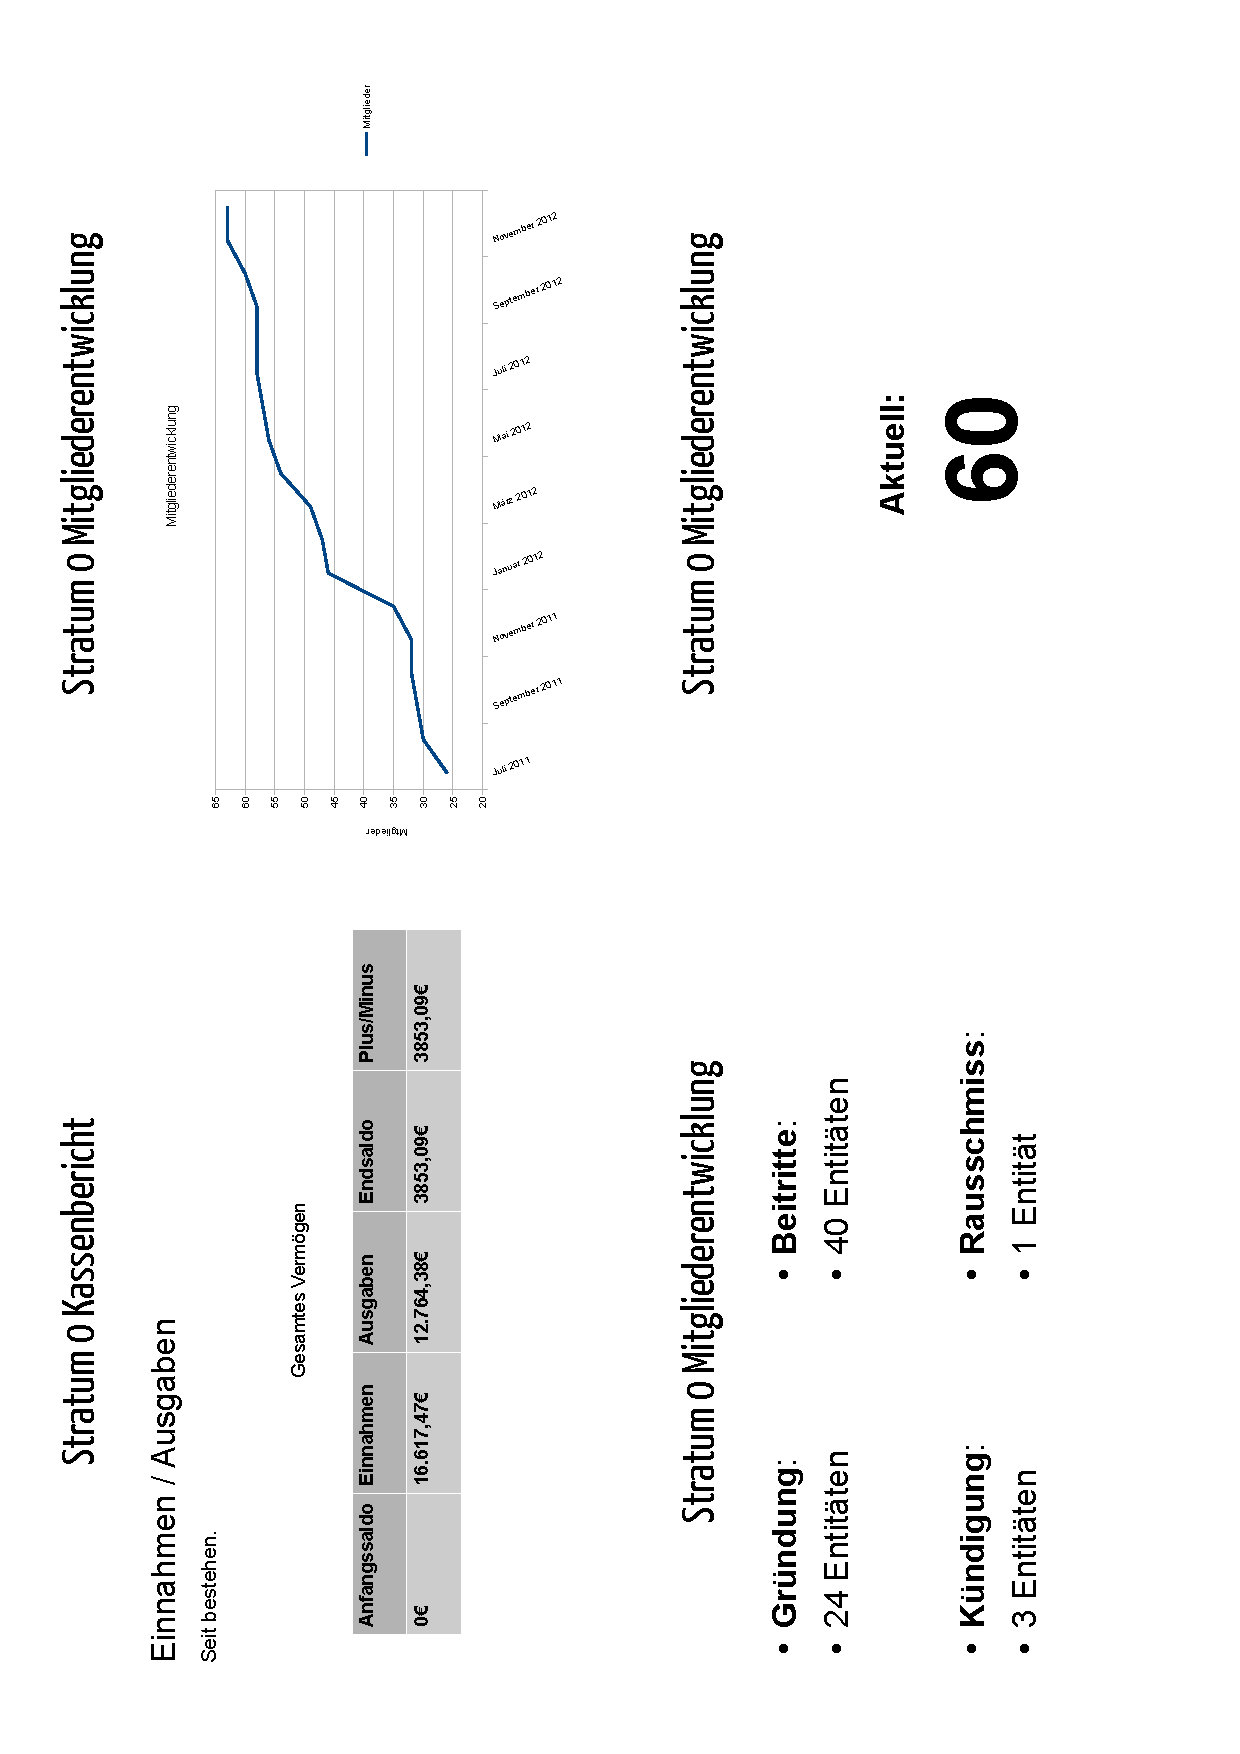
\includegraphics[height=\textheight]{images/Kassenbericht_2012_2.pdf}

%%%%%%%%%%%%%%%%%%%%
%% Unterschriften %%
%%%%%%%%%%%%%%%%%%%%
\cleardoublepage
\section*{Unterschriften}
\vspace{0.7cm}
\noindent Protokollführer: \hrulefill\hfill\phantom{c}\par
\vspace{0.7cm}
\noindent Vorstandsvorsitzender: \hrulefill\hfill\phantom{c}\par
\vspace{0.7cm}
\noindent Stellv. Vorsitzender: \hrulefill\hfill\phantom{c}\par
\vspace{0.7cm}
\noindent Schatzmeister: \hrulefill\hfill\phantom{c}\par
\vspace{0.7cm}
\noindent Beisitzer: \hrulefill\hfill\phantom{c}\par
\vspace{0.7cm}
\noindent Beisitzer: \hrulefill\hfill\phantom{c}\par
%\vspace{0.7cm}
%\noindent Beisitzer: \hrulefill\hfill\phantom{c}\par

\end{document}
